\documentclass[aspectratio=169, 10pt]{beamer}

% Modern professional theme
\usetheme{metropolis}
\usepackage{appendixnumberbeamer}

% Color palette
\definecolor{deepblue}{RGB}{23, 42, 69}
\definecolor{vibrantblue}{RGB}{52, 152, 219}
\definecolor{softwhite}{RGB}{248, 249, 250}
\definecolor{warmgold}{RGB}{241, 196, 15}
\definecolor{coral}{RGB}{231, 76, 60}
\definecolor{emerald}{RGB}{46, 204, 113}
\definecolor{purple}{RGB}{155, 89, 182}
\definecolor{teal}{RGB}{26, 188, 156}
\definecolor{darkpurple}{RGB}{102, 51, 153}
\definecolor{sunset}{RGB}{255, 128, 0}

% Theme colors
\setbeamercolor{normal text}{fg=deepblue, bg=softwhite}
\setbeamercolor{alerted text}{fg=coral}
\setbeamercolor{frametitle}{bg=deepblue, fg=softwhite}
\setbeamercolor{progress bar}{fg=warmgold, bg=deepblue!30}
\setbeamercolor{block title}{bg=vibrantblue, fg=softwhite}
\setbeamercolor{block body}{bg=vibrantblue!10}

\setbeamertemplate{navigation symbols}{}
\setbeamertemplate{footline}[frame number]

% Packages
\usepackage{graphicx}
\usepackage{tikz}
\usepackage{pgfplots}
\usepackage{fontawesome5}
\usepackage{tcolorbox}
\usepackage{booktabs}
\usepackage{amsmath}
\usepackage{listings}
\usepackage{xcolor}
\usepackage{hyperref}

\usetikzlibrary{shapes.geometric, arrows, positioning, calc, decorations.pathreplacing, fit}
\pgfplotsset{compat=1.18}

% Reusable tikz styles
\tikzset{
  treenode/.style={circle, draw=#1, fill=#1!15, minimum size=0.7cm, font=\small\bfseries, line width=1.2pt},
  leafnode/.style={rectangle, draw=#1, fill=#1!12, rounded corners=2pt, minimum width=0.8cm, minimum height=0.6cm, font=\small\bfseries, line width=1.2pt},
  intnode/.style={circle, draw=deepblue!60, fill=deepblue!8, minimum size=0.65cm, font=\small},
  edgelabel/.style={font=\scriptsize\bfseries, text=#1},
}

% Code listing style
\lstset{
  basicstyle=\ttfamily\tiny,
  backgroundcolor=\color{deepblue!5},
  frame=single,
  rulecolor=\color{deepblue!30},
  keywordstyle=\color{vibrantblue}\bfseries,
  stringstyle=\color{emerald},
  commentstyle=\color{deepblue!50}\itshape,
  breaklines=true,
  showstringspaces=false
}

% Custom boxes
\newtcolorbox{infobox}[1][]{colback=vibrantblue!8, colframe=vibrantblue, title=#1, fonttitle=\bfseries, arc=2mm}
\newtcolorbox{warnbox}[1][]{colback=coral!8, colframe=coral, title=#1, fonttitle=\bfseries, arc=2mm}
\newtcolorbox{tipbox}[1][]{colback=emerald!8, colframe=emerald, title=#1, fonttitle=\bfseries, arc=2mm}
\newtcolorbox{workshopbox}[1][]{colback=purple!8, colframe=purple, title=#1, fonttitle=\bfseries, arc=2mm}
\newtcolorbox{casebox}[1][]{colback=sunset!8, colframe=sunset, title=#1, fonttitle=\bfseries, arc=2mm}
\newtcolorbox{problembox}[1][]{colback=coral!6, colframe=coral!80, title=#1, fonttitle=\bfseries, arc=2mm}
\newtcolorbox{solutionbox}[1][]{colback=emerald!6, colframe=emerald!80, title=#1, fonttitle=\bfseries, arc=2mm}

% Title info
\title{Huffman Coding}
\subtitle{Class 4 --- Optimal Prefix-Free Codes}
\author{Data Compression}
\date{Spring 2026}

\begin{document}

% ============================================================
% TITLE SLIDE
% ============================================================
{
\setbeamercolor{background canvas}{bg=deepblue}
\begin{frame}[plain]
\begin{center}
\textcolor{warmgold}{\fontsize{36}{42}\bfseries\selectfont Huffman Coding}\\[0.5cm]
\textcolor{softwhite}{\Large Optimal Prefix-Free Variable-Length Codes}\\[0.3cm]
\textcolor{softwhite!60}{\normalsize Data Compression --- Class 4}\\[0.6cm]
\textcolor{softwhite!30}{\fontsize{32}{38}\selectfont\faTree\quad\faCompress\quad\faFileCode\quad\faChartBar}\\[0.5cm]
\textcolor{softwhite!50}{\small Spring 2026}
\end{center}
\end{frame}
}

% ============================================================
% AGENDA
% ============================================================
\begin{frame}{Today's Roadmap}
\begin{columns}[T]
\begin{column}{0.48\textwidth}
\textcolor{coral}{\faLayerGroup\ \textbf{Part 1: Foundations}}
\begin{itemize}\setlength\itemsep{0pt}
\item Why variable-length codes?
\item Prefix-free property
\item Information \& Entropy recap
\end{itemize}

\vspace{0.2cm}
\textcolor{vibrantblue}{\faTree\ \textbf{Part 2: Huffman Algorithm}}
\begin{itemize}\setlength\itemsep{0pt}
\item Greedy construction
\item Step-by-step examples (ABRACADABRA, HELLO)
\item Optimality \& Huffman vs Shannon--Fano
\end{itemize}
\end{column}
\begin{column}{0.48\textwidth}
\textcolor{emerald}{\faFlask\ \textbf{Part 3: Worked Examples}}
\begin{itemize}\setlength\itemsep{0pt}
\item BANANA, BOOKKEEPER, COCONUT
\item Encoding \& decoding walkthrough
\end{itemize}

\vspace{0.2cm}
\textcolor{purple}{\faGlobe\ \textbf{Part 4: Real-World Applications}}
\begin{itemize}\setlength\itemsep{0pt}
\item JPEG, PNG, DEFLATE, MP3
\item Adaptive \& Extended Huffman
\end{itemize}

\vspace{0.2cm}
\textcolor{sunset}{\faEdit\ \textbf{Part 5: Practice Problems}}
\begin{itemize}\setlength\itemsep{0pt}
\item Build trees, compute savings
\item Huffman vs Shannon--Fano
\end{itemize}
\end{column}
\end{columns}
\end{frame}

% ============================================================
% PART 1 HEADER
% ============================================================
{
\setbeamercolor{background canvas}{bg=coral}
\begin{frame}[plain]
\begin{center}
\textcolor{softwhite}{\Large Part 1}\\[0.3cm]
\textcolor{warmgold}{\fontsize{30}{36}\bfseries Foundations}\\[0.3cm]
\textcolor{softwhite!80}{\normalsize Why not just use ASCII?}
\end{center}
\end{frame}
}

% ============================================================
% FIXED vs VARIABLE LENGTH
% ============================================================
\begin{frame}{Fixed-Length vs Variable-Length Codes}
\begin{columns}
\begin{column}{0.48\textwidth}
\textcolor{coral}{\bfseries \faCube\ Fixed-Length (e.g.\ ASCII)}\\[0.2cm]
\begin{itemize}
\item Every symbol gets the \textbf{same} number of bits
\item ASCII: 8 bits per character, always
\item Simple but wasteful
\end{itemize}
\vspace{0.2cm}
\small Example: ``AAABBC'' in 3-bit fixed code\\
A=000, B=001, C=010\\
Encoded: \texttt{000 000 000 001 001 010}\\
Total: \textbf{18 bits}
\end{column}
\begin{column}{0.48\textwidth}
\textcolor{emerald}{\bfseries \faCompress\ Variable-Length}\\[0.2cm]
\begin{itemize}
\item Frequent symbols $\rightarrow$ \textbf{short} codes
\item Rare symbols $\rightarrow$ \textbf{long} codes
\item Matches the information content!
\end{itemize}
\vspace{0.2cm}
\small Same ``AAABBC'' with Huffman:\\
A=0, B=10, C=11\\
Encoded: \texttt{0 0 0 10 10 11}\\
Total: \textbf{10 bits} \textcolor{emerald}{(44\% savings!)}
\end{column}
\end{columns}
\vspace{0.15cm}
\begin{infobox}[\faLightbulb\ Key Insight]
\small Frequent symbols carry \textbf{less information} (less surprise). Give them shorter codes. This is the core idea behind Huffman coding.
\end{infobox}
\end{frame}

% ============================================================
% PREFIX-FREE PROPERTY
% ============================================================
\begin{frame}{The Prefix-Free Property: Why It Matters}
\begin{columns}
\begin{column}{0.5\textwidth}
\textbf{Problem with arbitrary variable-length codes:}\\[0.2cm]
\small Suppose A=0, B=01, C=1.\\
Bitstream \texttt{01} --- is it ``AB'' or ``B''?\\[0.1cm]
\textcolor{coral}{\bfseries Ambiguous! Can't decode uniquely.}\\[0.3cm]

\textcolor{emerald}{\bfseries Prefix-free rule:}\\
No codeword is a \textbf{prefix} of another codeword.\\[0.2cm]
\small Example: A=0, B=10, C=11 \textcolor{emerald}{\faCheck}\\
\texttt{01011} $\rightarrow$ 0\,|\,10\,|\,11 $\rightarrow$ ``ABC'' \textcolor{emerald}{(unique!)}
\end{column}
\begin{column}{0.45\textwidth}
\begin{center}
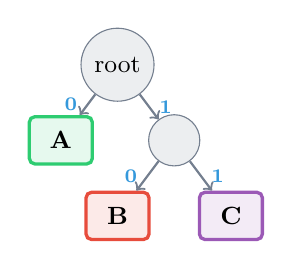
\begin{tikzpicture}[scale=0.8,
  level distance=1.2cm, sibling distance=1.8cm,
  edge from parent/.style={draw, thick, ->, deepblue!60}]
\node[intnode] {root}
  child {
    node[leafnode=emerald] {A}
    edge from parent node[left, edgelabel=vibrantblue] {0}
  }
  child {
    node[intnode] {}
    child {
      node[leafnode=coral] {B}
      edge from parent node[left, edgelabel=vibrantblue] {0}
    }
    child {
      node[leafnode=purple] {C}
      edge from parent node[right, edgelabel=vibrantblue] {1}
    }
    edge from parent node[right, edgelabel=vibrantblue] {1}
  };
\end{tikzpicture}\\[0.1cm]
\small\textcolor{deepblue!60}{Symbols only at \textbf{leaves} $\rightarrow$ prefix-free}
\end{center}
\end{column}
\end{columns}
\vspace{0.1cm}
\begin{tipbox}[\faTree\ Binary Tree Connection]
\small Any prefix-free code corresponds to a binary tree. Symbols at leaves, left edge = 0, right edge = 1. Huffman finds the \textbf{optimal} such tree.
\end{tipbox}
\end{frame}

% ============================================================
% ENTROPY RECAP
% ============================================================
\begin{frame}{Quick Recap: Information \& Entropy}
\begin{columns}
\begin{column}{0.5\textwidth}
\textcolor{vibrantblue}{\bfseries \faChartBar\ Shannon Information:}\\[0.1cm]
\small Information of symbol $s_i$ with probability $p_i$:\\[0.1cm]
$I(s_i) = -\log_2(p_i) \text{ bits}$\\[0.2cm]

\textcolor{coral}{\bfseries \faCalculator\ Entropy (average info):}\\[0.1cm]
$H = -\sum_{i} p_i \log_2(p_i) \text{ bits/symbol}$\\[0.2cm]

\textbf{Entropy is the theoretical minimum} average bits per symbol for lossless compression.\\[0.2cm]

\begin{warnbox}[\faExclamationTriangle\ Fundamental Limit]
\small No lossless code can achieve average length $<$ $H$. Huffman gets \textbf{closest} among symbol-by-symbol codes.
\end{warnbox}
\end{column}
\begin{column}{0.45\textwidth}
\begin{center}
\footnotesize
\textbf{Example: ``AABBAC'' (6 chars)}\\[0.1cm]
\begin{tabular}{cccc}
\toprule
Sym & Count & Prob & Info (bits) \\
\midrule
A & 3 & 0.5 & $-\log_2(0.5) = 1.0$ \\
B & 2 & $\frac{1}{3}$ & $-\log_2(\frac{1}{3}) = 1.58$ \\
C & 1 & $\frac{1}{6}$ & $-\log_2(\frac{1}{6}) = 2.58$ \\
\bottomrule
\end{tabular}\\[0.15cm]
$H = 0.5(1) + 0.33(1.58) + 0.17(2.58)$\\
$H = \textbf{1.46}$ bits/symbol\\[0.15cm]
\textcolor{emerald}{\small Huffman: A=0, B=10, C=11 $\rightarrow$ $\bar{L}=1.5$}
\end{center}
\end{column}
\end{columns}
\end{frame}

% ============================================================
% PART 2 HEADER
% ============================================================
{
\setbeamercolor{background canvas}{bg=vibrantblue}
\begin{frame}[plain]
\begin{center}
\textcolor{softwhite}{\Large Part 2}\\[0.3cm]
\textcolor{warmgold}{\fontsize{30}{36}\bfseries The Huffman Algorithm}\\[0.3cm]
\textcolor{softwhite!80}{\normalsize A Greedy Approach to Optimal Codes}
\end{center}
\end{frame}
}


% ============================================================
% ALGORITHM STEPS
% ============================================================
\begin{frame}{Huffman Algorithm: The Steps}
\begin{columns}
\begin{column}{0.5\textwidth}
\begin{workshopbox}[\faCog\ Algorithm]
\small
\begin{enumerate}\setlength\itemsep{1pt}
\item Create a \textbf{leaf node} for each symbol
\item Insert all into a \textbf{min-heap} (priority queue)
\item \textbf{While} queue size $>$ 1:
  \begin{enumerate}\setlength\itemsep{0pt}
  \item[a.] Remove \textbf{two lowest} frequency nodes
  \item[b.] Create internal node (freq = sum)
  \item[c.] Attach as left/right children
  \item[d.] Insert new node back
  \end{enumerate}
\item Remaining node = \textbf{root}
\end{enumerate}
\end{workshopbox}
\end{column}
\begin{column}{0.45\textwidth}
\begin{infobox}[\faLightbulb\ Why Greedy Works]
\small Least frequent symbols get the \textbf{longest} codes (deepest in tree). Merging them first guarantees this. Greedy $\rightarrow$ globally optimal!
\end{infobox}
\vspace{0.1cm}
\begin{tipbox}[\faClock\ Complexity]
\small $O(n \log n)$ --- dominated by heap operations.
\end{tipbox}
\end{column}
\end{columns}
\end{frame}

% ============================================================
% STEP-BY-STEP EXAMPLE
% ============================================================
\begin{frame}{Step-by-Step: Building a Huffman Tree}
\small\textbf{Message:} ``ABRACADABRA'' \quad Frequencies: A=5, B=2, R=2, C=1, D=1\\[0.15cm]
\begin{center}
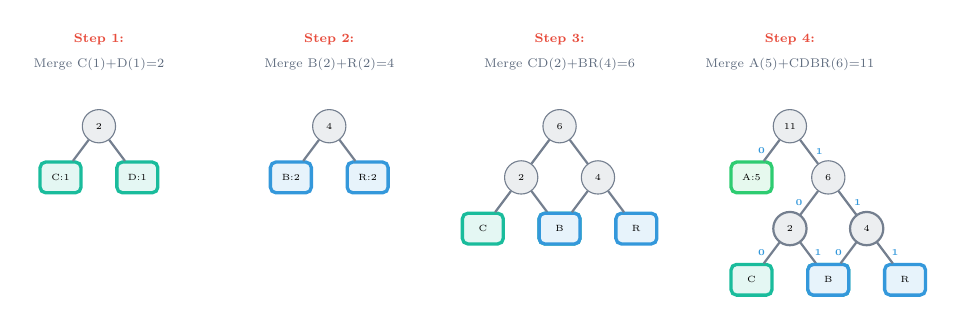
\begin{tikzpicture}[scale=0.65, transform shape,
  level distance=1cm, sibling distance=1.5cm,
  edge from parent/.style={draw, thick, deepblue!60}]

% Step labels
\node[font=\scriptsize\bfseries, text=coral] at (-1,0.5) {Step 1:};
\node[font=\scriptsize, text=deepblue!70] at (-1,0) {Merge C(1)+D(1)=2};

\node[font=\scriptsize\bfseries, text=coral] at (3.5,0.5) {Step 2:};
\node[font=\scriptsize, text=deepblue!70] at (3.5,0) {Merge B(2)+R(2)=4};

\node[font=\scriptsize\bfseries, text=coral] at (8,0.5) {Step 3:};
\node[font=\scriptsize, text=deepblue!70] at (8,0) {Merge CD(2)+BR(4)=6};

\node[font=\scriptsize\bfseries, text=coral] at (12.5,0.5) {Step 4:};
\node[font=\scriptsize, text=deepblue!70] at (12.5,0) {Merge A(5)+CDBR(6)=11};

% Step 1 mini tree
\node[intnode] at (-1,-1.2) {\tiny 2}
  child { node[leafnode=teal, font=\tiny] {C\tiny:1} }
  child { node[leafnode=teal, font=\tiny] {D\tiny:1} };

% Step 2 mini tree
\node[intnode] at (3.5,-1.2) {\tiny 4}
  child { node[leafnode=vibrantblue, font=\tiny] {B\tiny:2} }
  child { node[leafnode=vibrantblue, font=\tiny] {R\tiny:2} };

% Step 3 mini tree
\node[intnode] at (8,-1.2) {\tiny 6}
  child {
    node[intnode] {\tiny 2}
    child { node[leafnode=teal, font=\tiny] {C} }
    child { node[leafnode=teal, font=\tiny] {D} }
  }
  child {
    node[intnode] {\tiny 4}
    child { node[leafnode=vibrantblue, font=\tiny] {B} }
    child { node[leafnode=vibrantblue, font=\tiny] {R} }
  };

% Step 4 final tree
\node[intnode] at (12.5,-1.2) {\tiny 11}
  child {
    node[leafnode=emerald, font=\tiny] {A\tiny:5}
    edge from parent node[left, font=\tiny\bfseries, text=vibrantblue] {0}
  }
  child {
    node[intnode] {\tiny 6}
    child {
      node[intnode] {\tiny 2}
      child { node[leafnode=teal, font=\tiny] {C} edge from parent node[left, font=\tiny\bfseries, text=vibrantblue] {0} }
      child { node[leafnode=teal, font=\tiny] {D} edge from parent node[right, font=\tiny\bfseries, text=vibrantblue] {1} }
      edge from parent node[left, font=\tiny\bfseries, text=vibrantblue] {0}
    }
    child {
      node[intnode] {\tiny 4}
      child { node[leafnode=vibrantblue, font=\tiny] {B} edge from parent node[left, font=\tiny\bfseries, text=vibrantblue] {0} }
      child { node[leafnode=vibrantblue, font=\tiny] {R} edge from parent node[right, font=\tiny\bfseries, text=vibrantblue] {1} }
      edge from parent node[right, font=\tiny\bfseries, text=vibrantblue] {1}
    }
    edge from parent node[right, font=\tiny\bfseries, text=vibrantblue] {1}
  };
\end{tikzpicture}
\end{center}
\vspace{0.05cm}
\begin{casebox}[title={\faTable\ Result: A=0 | B=110 | R=111 | C=100 | D=101}]
\small ``ABRACADABRA'' $\rightarrow$ \texttt{0\,110\,111\,0\,100\,0\,101\,0\,110\,111\,0} = \textbf{23 bits} vs 33 bits fixed (3-bit) = \textcolor{emerald}{\bfseries 30\% savings}
\end{casebox}
\end{frame}

% ============================================================
% TEXTBOOK EXAMPLE: HELLO
% ============================================================
\begin{frame}{Textbook Example: Coding ``HELLO''}
\begin{columns}
\begin{column}{0.48\textwidth}
\small\textbf{Message:} ``HELLO'' \quad Freq: L=2, H=1, E=1, O=1\\[0.1cm]
\textbf{Algorithm 7.1 trace:}\\[0.05cm]
\footnotesize
\begin{tabular}{cl}
\toprule
Step & List contents \\
\midrule
Init & L(2), H(1), E(1), O(1) \\
1 & Merge E(1)+O(1) $\rightarrow$ P1(2) \\
2 & Merge H(1)+P1(2) $\rightarrow$ P2(3) \\
3 & Merge L(2)+P2(3) $\rightarrow$ P3(5) \\
\bottomrule
\end{tabular}
\vspace{0.1cm}

\small\textbf{Codes:} L=0, H=10, E=110, O=111\\[0.05cm]
\textbf{Avg bits/char:} $(1+1+2+3+3)/5 = \textbf{2.0}$\\[0.05cm]
\textbf{Fixed 3-bit:} $5 \times 3 = 15$ bits\\
\textbf{Huffman:} $1+1+2+3+3 = \textbf{10}$ bits \textcolor{emerald}{(33\% saved)}
\end{column}
\begin{column}{0.48\textwidth}
\begin{center}
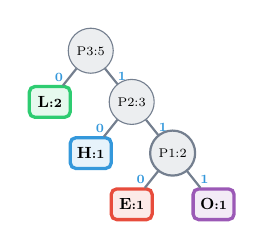
\begin{tikzpicture}[scale=0.65, transform shape,
  level distance=1cm, sibling distance=1.6cm,
  edge from parent/.style={draw, thick, deepblue!60}]
\node[intnode] {\scriptsize P3:5}
  child {
    node[leafnode=emerald] {\textbf{L}\scriptsize:2}
    edge from parent node[left, edgelabel=vibrantblue] {0}
  }
  child {
    node[intnode] {\scriptsize P2:3}
    child {
      node[leafnode=vibrantblue] {\textbf{H}\scriptsize:1}
      edge from parent node[left, edgelabel=vibrantblue] {0}
    }
    child {
      node[intnode] {\scriptsize P1:2}
      child {
        node[leafnode=coral] {\textbf{E}\scriptsize:1}
        edge from parent node[left, edgelabel=vibrantblue] {0}
      }
      child {
        node[leafnode=purple] {\textbf{O}\scriptsize:1}
        edge from parent node[right, edgelabel=vibrantblue] {1}
      }
      edge from parent node[right, edgelabel=vibrantblue] {1}
    }
    edge from parent node[right, edgelabel=vibrantblue] {1}
  };
\end{tikzpicture}
\end{center}
\vspace{0.05cm}
\begin{infobox}[\faLightbulb\ Observation]
\small L appears most (2$\times$) $\rightarrow$ shortest code (1 bit). E and O are rarest $\rightarrow$ longest (3 bits). Frequent symbols naturally get shorter codes.
\end{infobox}
\end{column}
\end{columns}
\end{frame}

% ============================================================
% OPTIMALITY
% ============================================================
\begin{frame}{Why Huffman Is Optimal}
\begin{columns}
\begin{column}{0.5\textwidth}
\textcolor{vibrantblue}{\bfseries \faAward\ Optimality Theorem}\\[0.1cm]
\small Among all prefix-free codes, Huffman produces the \textbf{minimum average codeword length}.\\[0.15cm]

\textbf{Key properties (proven in [Huffman 1952]):}
\begin{enumerate}\setlength\itemsep{0pt}
\item Two least-frequent symbols have \textbf{same-length} codes, differing only at the last bit
\item If $p_i \geq p_j$ then $l_i \leq l_j$ --- more frequent $\rightarrow$ shorter code
\item Average code length satisfies: $H \leq \bar{L} < H + 1$
\end{enumerate}
\vspace{0.1cm}
\small\textbf{Proof idea:} In any optimal tree, the two least-frequent symbols must be siblings at maximum depth. Merging them reduces to a smaller subproblem --- induction completes the proof.
\end{column}
\begin{column}{0.45\textwidth}
\begin{infobox}[\faChartLine\ How Close to Entropy?]
\small $H \leq \bar{L}_{\text{Huffman}} < H + 1$\\[0.1cm]
Within \textbf{1 bit} of entropy. When probabilities are powers of 2, Huffman \textbf{achieves $H$ exactly}.
\end{infobox}
\vspace{0.1cm}
\begin{tipbox}[\faLightbulb\ Note]
\small Huffman is optimal per-symbol. \textbf{Arithmetic coding} approaches $H$ without the +1 gap.
\end{tipbox}
\end{column}
\end{columns}
\end{frame}


% ============================================================
% HUFFMAN vs SHANNON-FANO
% ============================================================
\begin{frame}{Huffman vs Shannon--Fano}
\begin{columns}
\begin{column}{0.48\textwidth}
\textcolor{coral}{\bfseries \faArrowDown\ Shannon--Fano (Top-Down)}\\[0.1cm]
\small Divide symbols into two groups of roughly equal total probability. Assign 0/1 to each group. Recurse.\\[0.1cm]
\footnotesize
\textbf{Word:} ``ABRACADABRA'' --- A(5), B(2), R(2), C(1), D(1)\\[0.05cm]
Split: \{A\}=5 vs \{B,R,C,D\}=6\\
Then \{B,R\}=4 vs \{C,D\}=2\\[0.1cm]
\small Result: A=0, B=10, R=11, C=110, D=111\\
Total: $5(1)+2(2)+2(2)+1(3)+1(3) = \textbf{19}$\\[0.15cm]

\textcolor{emerald}{\bfseries \faArrowUp\ Huffman (Bottom-Up)}\\[0.1cm]
\small Merge two lowest-frequency nodes repeatedly.\\[0.1cm]
\footnotesize
Result: A=0, B=110, R=111, C=100, D=101\\
Total: $5(1)+2(3)+2(3)+1(3)+1(3) = \textbf{23}$
\end{column}
\begin{column}{0.48\textwidth}
\begin{center}
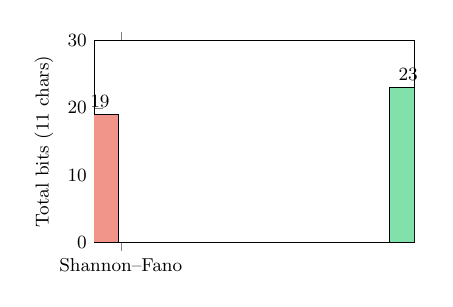
\begin{tikzpicture}[scale=0.75]
\begin{axis}[
    ybar, bar width=18pt,
    ylabel={\small Total bits (11 chars)},
    symbolic x coords={Shannon--Fano,Huffman},
    xtick=data, ymin=0, ymax=30,
    tick label style={font=\small},
    ylabel style={font=\small},
    width=7cm, height=5cm,
    nodes near coords, every node near coord/.append style={font=\small\bfseries}
]
\addplot[fill=coral!60] coordinates {(Shannon--Fano,19)};
\addplot[fill=emerald!60] coordinates {(Huffman,23)};
\end{axis}
\end{tikzpicture}
\end{center}
\vspace{0.05cm}
\begin{tipbox}[\faLightbulb\ Key Difference]
\small Shannon--Fano is \textbf{not guaranteed optimal}. Huffman \textbf{always} produces minimum average code length. Ties in the queue can yield different valid trees.
\end{tipbox}
\end{column}
\end{columns}
\end{frame}

% ============================================================
% PART 3 HEADER
% ============================================================
{
\setbeamercolor{background canvas}{bg=emerald}
\begin{frame}[plain]
\begin{center}
\textcolor{softwhite}{\Large Part 3}\\[0.3cm]
\textcolor{warmgold}{\fontsize{30}{36}\bfseries Worked Examples}\\[0.3cm]
\textcolor{softwhite!80}{\normalsize Let's build some trees}
\end{center}
\end{frame}
}

% ============================================================
% WORKED EXAMPLE 1: BANANA
% ============================================================
\begin{frame}{Worked Example 1: Coding ``BANANA''}
\begin{columns}
\begin{column}{0.45\textwidth}
\small\textbf{Message:} ``BANANA'' (6 chars)\\
Frequencies: A=3, N=2, B=1\\[0.1cm]
\footnotesize
\begin{tabular}{ccccc}
\toprule
Sym & Count & Prob & Code & Bits \\
\midrule
A & 3 & 0.50 & 0 & 1 \\
N & 2 & 0.33 & 10 & 2 \\
B & 1 & 0.17 & 11 & 2 \\
\bottomrule
\end{tabular}
\vspace{0.15cm}

\small\textbf{Merges:} B(1)+N(2)=BN(3), then A(3)+BN(3)=root(6)\\[0.1cm]
\textbf{Average code length:}\\
$\bar{L} = 0.5(1) + 0.33(2) + 0.17(2) = \textbf{1.5}$ bits/sym\\[0.1cm]
\textbf{Encode ``BANANA'':}\\
\texttt{11\,0\,10\,0\,10\,0} = \textbf{9 bits}\\
Fixed 2-bit: $6 \times 2 = 12$ bits. \textcolor{emerald}{\bfseries Saves 25\%}
\end{column}
\begin{column}{0.5\textwidth}
\begin{center}
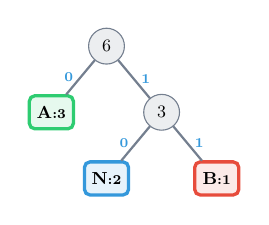
\begin{tikzpicture}[scale=0.7, transform shape,
  level distance=1.2cm, sibling distance=2cm,
  edge from parent/.style={draw, thick, deepblue!60}]
\node[intnode] {6}
  child {
    node[leafnode=emerald] {\textbf{A}\scriptsize:3}
    edge from parent node[left, edgelabel=vibrantblue] {0}
  }
  child {
    node[intnode] {3}
    child { node[leafnode=vibrantblue] {\textbf{N}\scriptsize:2} edge from parent node[left, edgelabel=vibrantblue] {0} }
    child { node[leafnode=coral] {\textbf{B}\scriptsize:1} edge from parent node[right, edgelabel=vibrantblue] {1} }
    edge from parent node[right, edgelabel=vibrantblue] {1}
  };
\end{tikzpicture}
\end{center}
\vspace{0.1cm}
\small Entropy: $H = 1.459$ bits/sym\\
$\bar{L} = 1.5$ (within 1 bit of $H$)\\[0.1cm]
\textcolor{emerald}{\bfseries Efficiency: $H/\bar{L} = 97.3\%$}
\begin{tipbox}[\faLightbulb\ Note]
\small A appears most $\rightarrow$ gets 1-bit code. B is rarest $\rightarrow$ gets 2-bit code. Classic Huffman behavior.
\end{tipbox}
\end{column}
\end{columns}
\end{frame}

% ============================================================
% WORKED EXAMPLE 2: BOOKKEEPER
% ============================================================
\begin{frame}{Worked Example 2: Coding ``BOOKKEEPER''}
\begin{columns}
\begin{column}{0.48\textwidth}
\small\textbf{Message:} ``BOOKKEEPER'' (10 chars)\\
Freq: E=2, O=2, K=2, B=1, P=1, R=1\\[0.1cm]
\footnotesize
\begin{tabular}{cccc}
\toprule
Sym & Count & Code & Bits \\
\midrule
E & 2 & 00 & 2 \\
O & 2 & 01 & 2 \\
K & 2 & 10 & 2 \\
B & 1 & 110 & 3 \\
P & 1 & 1110 & 4 \\
R & 1 & 1111 & 4 \\
\bottomrule
\end{tabular}
\vspace{0.1cm}

\small\textbf{Merges:} P(1)+R(1)=2, B(1)+PR(2)=3,\\
E(2)+O(2)=4, K(2)+BPR(3)=5, EO(4)+KBPR(5)=9\\[0.1cm]
\textbf{Encode ``BOOKKEEPER'':}\\
\footnotesize\texttt{110\,01\,01\,10\,10\,00\,00\,1110\,00\,1111} = \textbf{25 bits}\\
\small Fixed 3-bit: $10 \times 3 = 30$ bits. \textcolor{emerald}{\bfseries Saves 17\%}
\end{column}
\begin{column}{0.48\textwidth}
\begin{center}
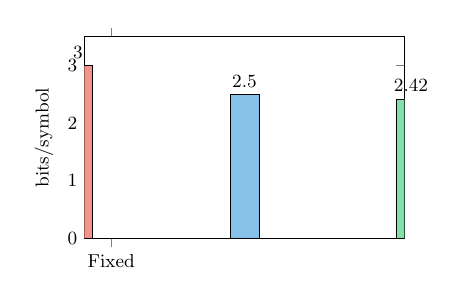
\begin{tikzpicture}[scale=0.75]
\begin{axis}[
    ybar, bar width=14pt,
    ylabel={\small bits/symbol},
    symbolic x coords={Fixed,Huffman,Entropy},
    xtick=data, ymin=0, ymax=3.5,
    tick label style={font=\small},
    ylabel style={font=\small},
    width=7cm, height=5cm,
    nodes near coords, every node near coord/.append style={font=\small}
]
\addplot[fill=coral!60] coordinates {(Fixed,3.0)};
\addplot[fill=vibrantblue!60] coordinates {(Huffman,2.5)};
\addplot[fill=emerald!60] coordinates {(Entropy,2.42)};
\end{axis}
\end{tikzpicture}
\end{center}
\vspace{0.1cm}
\begin{casebox}[\faLightbulb\ Observation]
\small With 6 distinct symbols in 10 characters, the distribution is fairly uniform. Huffman still saves 17\%, but the gap to entropy is larger when frequencies are similar.
\end{casebox}
\end{column}
\end{columns}
\end{frame}

% ============================================================
% WORKED EXAMPLE 3: ENCODING & DECODING COCONUT
% ============================================================
\begin{frame}{Worked Example 3: Encoding \& Decoding ``COCONUT''}
\begin{columns}
\begin{column}{0.48\textwidth}
\textcolor{vibrantblue}{\bfseries \faLock\ Encoding}\\[0.1cm]
\small\textbf{Message:} ``COCONUT'' (7 chars)\\
Freq: C=2, O=2, N=1, U=1, T=1\\[0.1cm]
\textbf{Codes:} C=00, O=01, N=10, U=110, T=111\\[0.1cm]
\textbf{Encode ``COCONUT'':}\\[0.05cm]
\footnotesize
\begin{tabular}{cl}
C $\rightarrow$ \texttt{00} & O $\rightarrow$ \texttt{01} \\
C $\rightarrow$ \texttt{00} & O $\rightarrow$ \texttt{01} \\
N $\rightarrow$ \texttt{10} & U $\rightarrow$ \texttt{110} \\
T $\rightarrow$ \texttt{111} & \\
\end{tabular}\\[0.05cm]
\small Bitstream: \texttt{00010001101101111} (\textbf{17 bits})\\
Fixed 3-bit: $7 \times 3 = 21$ bits. \textcolor{emerald}{Saves 19\%}
\end{column}
\begin{column}{0.48\textwidth}
\textcolor{coral}{\bfseries \faUnlock\ Decoding}\\[0.1cm]
\small Bitstream: \texttt{00010001101101111}\\
Walk tree from root, output at leaf, restart.\\[0.05cm]
\footnotesize
\begin{tabular}{cl}
\texttt{0,0} $\rightarrow$ C & \texttt{0,1} $\rightarrow$ O \\
\texttt{0,0} $\rightarrow$ C & \texttt{0,1} $\rightarrow$ O \\
\texttt{1,0} $\rightarrow$ N & \texttt{1,1,0} $\rightarrow$ U \\
\texttt{1,1,1} $\rightarrow$ T & \\
\end{tabular}\\[0.05cm]
\small Result: \textbf{COCONUT} \textcolor{emerald}{\faCheck}
\vspace{0.1cm}
\begin{tipbox}[\faLightbulb\ Key Point]
\small Prefix-free $\rightarrow$ decoding is \textbf{unambiguous}. Just walk the tree bit by bit. No lookahead needed.
\end{tipbox}
\end{column}
\end{columns}
\end{frame}


% ============================================================
% PART 4 HEADER
% ============================================================
{
\setbeamercolor{background canvas}{bg=purple}
\begin{frame}[plain]
\begin{center}
\textcolor{softwhite}{\Large Part 4}\\[0.3cm]
\textcolor{warmgold}{\fontsize{30}{36}\bfseries Real-World Applications}\\[0.3cm]
\textcolor{softwhite!80}{\normalsize Huffman is everywhere}
\end{center}
\end{frame}
}

% ============================================================
% JPEG
% ============================================================
\begin{frame}{Huffman in JPEG Image Compression}
\begin{columns}
\begin{column}{0.5\textwidth}
\textbf{JPEG pipeline (simplified):}
\begin{enumerate}\setlength\itemsep{1pt}
\item Split image into 8$\times$8 blocks
\item Apply \textbf{DCT} (Discrete Cosine Transform)
\item \textbf{Quantize} DCT coefficients (lossy step)
\item \textbf{Huffman encode} the quantized values
\end{enumerate}
\vspace{0.15cm}
\small After quantization, most coefficients are \textbf{zero} or small values. Huffman exploits this skewed distribution perfectly.\\[0.1cm]
\textcolor{deepblue!60}{\footnotesize JPEG uses predefined Huffman tables (Annex K) but also supports custom tables optimized per image.}
\end{column}
\begin{column}{0.45\textwidth}
\begin{center}
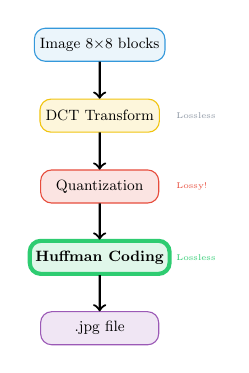
\begin{tikzpicture}[scale=0.6, transform shape,
  block/.style={draw=vibrantblue, fill=vibrantblue!10, rounded corners, minimum width=2.5cm, minimum height=0.7cm, font=\small, align=center}]
\node[block] (img) at (0,5) {Image 8$\times$8 blocks};
\node[block, fill=warmgold!15, draw=warmgold] (dct) at (0,3.5) {DCT Transform};
\node[block, fill=coral!15, draw=coral] (quant) at (0,2) {Quantization};
\node[block, fill=emerald!15, draw=emerald, line width=1.5pt] (huff) at (0,0.5) {\textbf{Huffman Coding}};
\node[block, fill=purple!15, draw=purple] (out) at (0,-1) {.jpg file};

\draw[->, thick] (img) -- (dct);
\draw[->, thick] (dct) -- (quant);
\draw[->, thick] (quant) -- (huff);
\draw[->, thick] (huff) -- (out);

\node[right, font=\tiny, text=deepblue!50] at (1.5,3.5) {Lossless};
\node[right, font=\tiny, text=coral] at (1.5,2) {Lossy!};
\node[right, font=\tiny, text=emerald] at (1.5,0.5) {Lossless};
\end{tikzpicture}
\end{center}
\end{column}
\end{columns}
\end{frame}

% ============================================================
% PNG, DEFLATE, MP3
% ============================================================
\begin{frame}{Huffman Everywhere: PNG, DEFLATE, MP3 \& More}
\begin{columns}[T]
\begin{column}{0.32\textwidth}
\begin{center}
\textcolor{vibrantblue}{\fontsize{20}{24}\selectfont\faImage}\\[0.1cm]
\textbf{PNG}\\[0.1cm]
\small Lossless image format. Uses DEFLATE = LZ77 + Huffman. Prediction filter $\rightarrow$ DEFLATE compress.\\[0.1cm]
\textcolor{deepblue!50}{\tiny Every PNG you've ever seen uses Huffman.}
\end{center}
\end{column}
\begin{column}{0.32\textwidth}
\begin{center}
\textcolor{emerald}{\fontsize{20}{24}\selectfont\faFileArchive}\\[0.1cm]
\textbf{DEFLATE / ZIP / GZIP}\\[0.1cm]
\small The backbone of web compression. LZ77 finds repeated patterns, then Huffman encodes the output.\\[0.1cm]
\textcolor{deepblue!50}{\tiny HTTP gzip, .zip files, .gz archives.}
\end{center}
\end{column}
\begin{column}{0.32\textwidth}
\begin{center}
\textcolor{purple}{\fontsize{20}{24}\selectfont\faMusic}\\[0.1cm]
\textbf{MP3 / AAC}\\[0.1cm]
\small Audio codecs. Psychoacoustic model removes inaudible frequencies, then Huffman encodes the rest.\\[0.1cm]
\textcolor{deepblue!50}{\tiny MP3 uses custom Huffman tables per frame.}
\end{center}
\end{column}
\end{columns}
\vspace{0.2cm}
\begin{infobox}[\faGlobe\ The Big Picture]
\small Huffman coding is a \textbf{building block} inside almost every compression format. It's rarely used alone --- it's the final entropy coding stage after domain-specific transforms (DCT, LZ77, psychoacoustic models).
\end{infobox}
\end{frame}

% ============================================================
% ADAPTIVE HUFFMAN & VARIANTS
% ============================================================
\begin{frame}{Adaptive Huffman \& Modern Variants}
\begin{columns}[T]
\begin{column}{0.48\textwidth}
\textcolor{coral}{\bfseries \faExclamationTriangle\ Problem with Static Huffman}\\[0.1cm]
\small You need to know symbol frequencies \textbf{before} encoding. This means:
\begin{itemize}\setlength\itemsep{0pt}
\item Two-pass: scan data, build tree, then encode
\item Must transmit the tree/table to the decoder
\item Table overhead can negate savings for small files
\end{itemize}
\vspace{0.15cm}
\textcolor{emerald}{\bfseries \faSync\ Adaptive Huffman (FGK / Vitter)}\\[0.1cm]
\small Update the tree \textbf{on-the-fly} as symbols arrive. Both encoder and decoder maintain identical trees. Single-pass, no table overhead.
\end{column}
\begin{column}{0.48\textwidth}
\textcolor{vibrantblue}{\bfseries \faChartLine\ Comparison}\\[0.1cm]
\footnotesize
\begin{tabular}{lcc}
\toprule
& \textbf{Static} & \textbf{Adaptive} \\
\midrule
Passes & 2 & 1 \\
Table overhead & Yes & No \\
Optimality & Optimal & Near-optimal \\
Complexity & $O(n \log n)$ & $O(n \log n)$ \\
Used in & JPEG, MP3 & Telecom \\
\bottomrule
\end{tabular}
\vspace{0.2cm}
\begin{tipbox}[\faArrowRight\ Modern Alternative]
\small Most modern formats now use \textbf{arithmetic coding} or \textbf{ANS} instead --- closer to entropy. Huffman remains popular due to simplicity.
\end{tipbox}
\end{column}
\end{columns}
\end{frame}

% ============================================================
% EXTENDED HUFFMAN CODING
% ============================================================
\begin{frame}{Extended Huffman Coding}
\begin{columns}
\begin{column}{0.48\textwidth}
\textcolor{coral}{\bfseries \faExclamationTriangle\ The Integer-Length Problem}\\[0.1cm]
\small Standard Huffman assigns each symbol an \textbf{integer} number of bits. But the ideal length $\log_2(1/p_i)$ is rarely an integer.\\[0.1cm]

\textbf{Example:} If $p = 0.9$, ideal = $0.15$ bits. Huffman must use at least \textbf{1 bit} --- huge waste!\\[0.15cm]

\textcolor{emerald}{\bfseries \faLayerGroup\ Solution: Block Symbols}\\[0.1cm]
\small Group $n$ symbols into blocks and build Huffman over all $n$-tuples. Per-symbol overhead shrinks:
$$H \leq \bar{L}_{\text{block}} < H + \frac{1}{n}$$
As $n \rightarrow \infty$, average length $\rightarrow$ entropy $H$.
\end{column}
\begin{column}{0.48\textwidth}
\begin{warnbox}[\faExclamationTriangle\ Trade-off]
\small Alphabet grows \textbf{exponentially}: $k^n$ entries. For $k=4$, $n=4$: 256 super-symbols. Practical limit on block size.
\end{warnbox}
\vspace{0.15cm}
\begin{tipbox}[\faArrowRight\ In Practice]
\small This motivated \textbf{arithmetic coding} --- it effectively achieves infinite block length without the exponential blowup.
\end{tipbox}
\end{column}
\end{columns}
\end{frame}

% ============================================================
% PART 5 HEADER
% ============================================================
{
\setbeamercolor{background canvas}{bg=sunset}
\begin{frame}[plain]
\begin{center}
\textcolor{softwhite}{\Large Part 5}\\[0.3cm]
\textcolor{deepblue}{\fontsize{30}{36}\bfseries Practice Problems}\\[0.3cm]
\textcolor{softwhite}{\normalsize Try before you peek at the solution!}
\end{center}
\end{frame}
}

% ============================================================
% PRACTICE PROBLEM 1: PINEAPPLE
% ============================================================
\begin{frame}{Practice Problem 1: Build a Huffman Tree}
\begin{problembox}[\faEdit\ Problem]
\small Build a Huffman code for the word ``PINEAPPLE'' (9 chars).\\[0.1cm]
\begin{center}
\begin{tabular}{ccccccc}
\toprule
Symbol & P & E & I & N & A & L \\
\midrule
Count & 3 & 2 & 1 & 1 & 1 & 1 \\
\bottomrule
\end{tabular}
\end{center}
\vspace{0.1cm}
\textbf{Tasks:}
\begin{enumerate}\setlength\itemsep{0pt}
\item Build the Huffman tree step by step
\item Write the Huffman code for each symbol
\item Calculate the average code length $\bar{L}$
\item Calculate entropy $H$ and compare with $\bar{L}$
\item Total bits for ``PINEAPPLE'': Huffman vs 3-bit fixed?
\end{enumerate}
\end{problembox}
\end{frame}

% ============================================================
% SOLUTION 1
% ============================================================
\begin{frame}{Solution 1: Huffman Tree for ``PINEAPPLE''}
\begin{columns}
\begin{column}{0.45\textwidth}
\small\textbf{Step-by-step merges:}\\[0.1cm]
\footnotesize
\begin{tabular}{cl}
\toprule
Step & Merge \\
\midrule
1 & A(1)+L(1) $\rightarrow$ AL(2) \\
2 & I(1)+N(1) $\rightarrow$ IN(2) \\
3 & E(2)+AL(2) $\rightarrow$ EAL(4) \\
4 & IN(2)+P(3) $\rightarrow$ INP(5) \\
5 & EAL(4)+INP(5) $\rightarrow$ root(9) \\
\bottomrule
\end{tabular}
\vspace{0.1cm}

\small\textbf{Codes:} P=11, E=00, I=100, N=101, A=010, L=011\\[0.05cm]
\textbf{Avg length:} $\bar{L} = \frac{3(2)+2(2)+1(3)+1(3)+1(3)+1(3)}{9} = \frac{22}{9} = \textbf{2.44}$\\[0.05cm]
\textbf{Entropy:} $H = 2.28$ bits/sym\\[0.05cm]
\textbf{``PINEAPPLE'':} Huffman = \textbf{22} bits\\
Fixed 3-bit: $9 \times 3 = 27$ bits. \textcolor{emerald}{Saves 19\%}
\end{column}
\begin{column}{0.5\textwidth}
\begin{center}
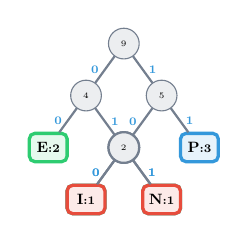
\begin{tikzpicture}[scale=0.6, transform shape,
  level distance=1.1cm, sibling distance=1.6cm,
  edge from parent/.style={draw, thick, deepblue!60}]
\node[intnode] {\tiny 9}
  child {
    node[intnode] {\tiny 4}
    child { node[leafnode=emerald] {\textbf{E}\scriptsize:2} edge from parent node[left, edgelabel=vibrantblue] {0} }
    child {
      node[intnode] {\tiny 2}
      child { node[leafnode=teal] {\textbf{A}\scriptsize:1} edge from parent node[left, edgelabel=vibrantblue] {0} }
      child { node[leafnode=teal] {\textbf{L}\scriptsize:1} edge from parent node[right, edgelabel=vibrantblue] {1} }
      edge from parent node[right, edgelabel=vibrantblue] {1}
    }
    edge from parent node[left, edgelabel=vibrantblue] {0}
  }
  child {
    node[intnode] {\tiny 5}
    child {
      node[intnode] {\tiny 2}
      child { node[leafnode=coral] {\textbf{I}\scriptsize:1} edge from parent node[left, edgelabel=vibrantblue] {0} }
      child { node[leafnode=coral] {\textbf{N}\scriptsize:1} edge from parent node[right, edgelabel=vibrantblue] {1} }
      edge from parent node[left, edgelabel=vibrantblue] {0}
    }
    child { node[leafnode=vibrantblue] {\textbf{P}\scriptsize:3} edge from parent node[right, edgelabel=vibrantblue] {1} }
    edge from parent node[right, edgelabel=vibrantblue] {1}
  };
\end{tikzpicture}
\end{center}
\end{column}
\end{columns}
\end{frame}

% ============================================================
% PRACTICE PROBLEM 2: TENNESSEE
% ============================================================
\begin{frame}{Practice Problem 2: Decode a Bitstream}
\begin{problembox}[\faEdit\ Problem]
\small The word ``TENNESSEE'' gives frequencies: E=4, N=2, S=2, T=1.\\
A Huffman tree produces codes: E=0, N=10, S=110, T=111.\\[0.1cm]
\textbf{Tasks:}
\begin{enumerate}\setlength\itemsep{0pt}
\item Draw the Huffman tree corresponding to these codes
\item Decode the bitstream: \texttt{111010100110011000}
\item Calculate $\bar{L}$ and $H$. How close is Huffman to entropy?
\item Encode ``TEEN'' and count total bits
\end{enumerate}
\end{problembox}
\end{frame}

% ============================================================
% SOLUTION 2
% ============================================================
\begin{frame}{Solution 2: Decoding ``TENNESSEE''}
\begin{columns}
\begin{column}{0.48\textwidth}
\textbf{1. Tree:}\\[0.1cm]
\begin{center}
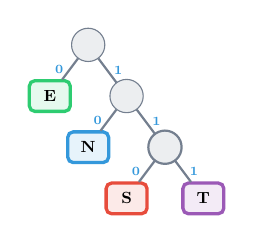
\begin{tikzpicture}[scale=0.65, transform shape,
  level distance=1cm, sibling distance=1.5cm,
  edge from parent/.style={draw, thick, deepblue!60}]
\node[intnode] {}
  child { node[leafnode=emerald] {\textbf{E}} edge from parent node[left, edgelabel=vibrantblue] {0} }
  child {
    node[intnode] {}
    child { node[leafnode=vibrantblue] {\textbf{N}} edge from parent node[left, edgelabel=vibrantblue] {0} }
    child {
      node[intnode] {}
      child { node[leafnode=coral] {\textbf{S}} edge from parent node[left, edgelabel=vibrantblue] {0} }
      child { node[leafnode=purple] {\textbf{T}} edge from parent node[right, edgelabel=vibrantblue] {1} }
      edge from parent node[right, edgelabel=vibrantblue] {1}
    }
    edge from parent node[right, edgelabel=vibrantblue] {1}
  };
\end{tikzpicture}
\end{center}
\vspace{0.1cm}
\textbf{2. Decode} \texttt{111010100110011000}:\\
\footnotesize 111|0|10|10|0|110|110|0|0 $\rightarrow$ \textbf{TENNESSEE}
\end{column}
\begin{column}{0.48\textwidth}
\textbf{3. Average length \& entropy:}\\[0.1cm]
\small $\bar{L} = \frac{4}{9}(1)+\frac{2}{9}(2)+\frac{2}{9}(3)+\frac{1}{9}(3)$\\
$= 0.44+0.44+0.67+0.33 = \textbf{1.89}$ bits/sym\\[0.1cm]
$H = 1.748$ bits/sym\\[0.1cm]
\begin{solutionbox}[\faCheck\ Observation]
\small $\bar{L} = 1.89$ vs $H = 1.748$. Huffman is within 0.14 bits of entropy --- \textbf{92.5\% efficient}. Not powers of 2, so a small gap exists.
\end{solutionbox}
\vspace{0.1cm}
\textbf{4. Encode ``TEEN'':}\\
\small 111\,|\,0\,|\,0\,|\,10 = \textbf{6 bits}
\end{column}
\end{columns}
\end{frame}

% ============================================================
% PRACTICE PROBLEM 3: ABRACADABRA COMPRESSION RATIO
% ============================================================
\begin{frame}{Practice Problem 3: Compression Ratio}
\begin{problembox}[\faEdit\ Problem]
\small A text file contains 10{,}000 repetitions of ``ABRACADABRA'' (110{,}000 chars total). Character frequencies from the word: A=5, B=2, R=2, C=1, D=1.\\[0.1cm]
\textbf{Tasks:}
\begin{enumerate}\setlength\itemsep{0pt}
\item Build the Huffman tree and assign codes
\item Total bits with Huffman vs fixed-length ($\lceil\log_2 5\rceil = 3$ bits)
\item Compression ratio (fixed / Huffman)?
\item Entropy $H$ and efficiency $\eta = H / \bar{L}$
\end{enumerate}
\end{problembox}
\end{frame}

% ============================================================
% SOLUTION 3
% ============================================================
\begin{frame}{Solution 3: Compression Ratio for ``ABRACADABRA''}
\begin{columns}
\begin{column}{0.48\textwidth}
\small\textbf{Freq per 11 chars:} A=5, B=2, R=2, C=1, D=1\\[0.1cm]
\textbf{Merges:} C(1)+D(1)=2, B(2)+R(2)=4, CD(2)+BR(4)=6, A(5)+CDBR(6)=11\\[0.1cm]
\textbf{Codes:}
\footnotesize
\begin{tabular}{cccc}
\toprule
Sym & Prob & Code & Len \\
\midrule
A & 5/11 & 0 & 1 \\
B & 2/11 & 110 & 3 \\
R & 2/11 & 111 & 3 \\
C & 1/11 & 100 & 3 \\
D & 1/11 & 101 & 3 \\
\bottomrule
\end{tabular}
\vspace{0.1cm}

\small\textbf{Avg length:} $\bar{L} = \frac{5(1)+2(3)+2(3)+1(3)+1(3)}{11} = \frac{23}{11} = \textbf{2.09}$
\end{column}
\begin{column}{0.48\textwidth}
\small\textbf{Total bits (110{,}000 chars):}\\
Huffman: $110{,}000 \times 2.09 = \textbf{229{,}900}$ bits\\
Fixed: $110{,}000 \times 3 = \textbf{330{,}000}$ bits\\[0.1cm]
\textbf{Compression ratio:} $330{,}000/229{,}900 = \textbf{1.44:1}$\\
\textcolor{emerald}{\bfseries Saves 100{,}100 bits (30.3\%)}\\[0.1cm]

\textbf{Entropy:} $H = 2.04$ bits/sym\\
\textbf{Efficiency:} $\eta = 2.04/2.09 = \textbf{97.6\%}$
\vspace{0.05cm}
\begin{solutionbox}[\faCheck\ Takeaway]
\small 97.6\% efficient --- Huffman is very close to the entropy bound for this skewed distribution.
\end{solutionbox}
\end{column}
\end{columns}
\end{frame}

% ============================================================
% PRACTICE PROBLEM 4: MISSISSIPPI
% ============================================================
\begin{frame}{Practice Problem 4: Longer Word Analysis}
\begin{problembox}[\faEdit\ Problem]
\small Build a Huffman code for ``MISSISSIPPI'' (11 chars).\\[0.1cm]
\begin{center}
\begin{tabular}{cccccc}
\toprule
Symbol & I & S & P & M \\
\midrule
Count & 4 & 4 & 2 & 1 \\
\bottomrule
\end{tabular}
\end{center}
\vspace{0.1cm}
\textbf{Tasks:}
\begin{enumerate}\setlength\itemsep{0pt}
\item Build the Huffman tree and assign codes
\item Encode ``MISSISSIPPI'' and count total bits
\item Fixed-length needs $\lceil\log_2 4\rceil = 2$ bits/char. Compare savings.
\item If this word repeats 1 million times, how many bytes does Huffman save vs fixed?
\end{enumerate}
\end{problembox}
\end{frame}

% ============================================================
% SOLUTION 4
% ============================================================
\begin{frame}{Solution 4: ``MISSISSIPPI'' Analysis}
\begin{columns}
\begin{column}{0.48\textwidth}
\small\textbf{Merges:} M(1)+P(2)=MP(3), then I(4)+S(4)=IS(8), then MP(3)+IS(8)=root(11)\\[0.1cm]
\textbf{Codes:}
\footnotesize
\begin{tabular}{cccc}
\toprule
Sym & Count & Code & Len \\
\midrule
I & 4 & 00 & 2 \\
S & 4 & 01 & 2 \\
P & 2 & 10 & 2 \\
M & 1 & 11 & 2 \\
\bottomrule
\end{tabular}
\vspace{0.1cm}

\small\textbf{Encode ``MISSISSIPPI'':}\\
\footnotesize\texttt{11\,00\,01\,01\,00\,01\,01\,00\,10\,10\,00} = \textbf{22 bits}\\[0.1cm]
\small Fixed 2-bit: $11 \times 2 = 22$ bits\\
\textcolor{coral}{\bfseries Same! No savings here.}
\end{column}
\begin{column}{0.48\textwidth}
\small\textbf{Why no savings?}\\[0.1cm]
With 4 symbols and fairly balanced frequencies, all codes end up 2 bits --- same as fixed-length.\\[0.1cm]

\textbf{Entropy:} $H = 1.748$ bits/sym\\
$\bar{L} = 2.0$ bits/sym\\
\textbf{Efficiency:} $87.4\%$\\[0.1cm]

\begin{solutionbox}[\faCheck\ Key Lesson]
\small Huffman helps most when frequencies are \textbf{highly skewed}. When symbols are roughly equally likely, fixed-length is already near-optimal. The gap $\bar{L} - H = 0.25$ bits is the ``integer penalty.''
\end{solutionbox}
\end{column}
\end{columns}
\end{frame}

% ============================================================
% PRACTICE PROBLEM 5: HUFFMAN vs SHANNON-FANO
% ============================================================
\begin{frame}{Practice Problem 5: Huffman vs Shannon--Fano}
\begin{problembox}[\faEdit\ Problem]
\small Consider the word ``ENGINEERING'' (11 chars).\\[0.1cm]
\begin{center}
\begin{tabular}{cccccccc}
\toprule
Symbol & E & N & G & I & R \\
\midrule
Count & 3 & 3 & 2 & 2 & 1 \\
\bottomrule
\end{tabular}
\end{center}
\vspace{0.1cm}
\textbf{Tasks:}
\begin{enumerate}\setlength\itemsep{0pt}
\item Build the Huffman tree and assign codes
\item Compute total bits to encode ``ENGINEERING'' with Huffman
\item Apply Shannon--Fano (top-down splitting) and assign codes
\item Compare total bits: which method wins?
\item Calculate entropy $H$ and compare both methods
\end{enumerate}
\end{problembox}
\end{frame}

% ============================================================
% SOLUTION 5
% ============================================================
\begin{frame}{Solution 5: ``ENGINEERING'' --- Huffman vs Shannon--Fano}
\begin{columns}
\begin{column}{0.48\textwidth}
\textcolor{emerald}{\bfseries \faTree\ Huffman (Bottom-Up):}\\[0.1cm]
\footnotesize
Merge: R(1)+G(2)=RG(3), I(2)+RG(3)=IRG(5), E(3)+N(3)=EN(6), IRG(5)+EN(6)=root(11)\\[0.1cm]
\small\textbf{Codes:} E=10, N=11, G=010, I=00, R=011\\
Total: $3(2)+3(2)+2(3)+2(2)+1(3) = \textbf{25}$ bits\\[0.15cm]

\textcolor{coral}{\bfseries \faArrowDown\ Shannon--Fano (Top-Down):}\\[0.1cm]
\footnotesize
Split: \{E,N\}=6 vs \{G,I,R\}=5\\
Then E=00, N=01, G=10, I=110, R=111\\[0.1cm]
\small Total: $3(2)+3(2)+2(2)+2(3)+1(3) = \textbf{25}$ bits\\[0.1cm]

\textcolor{vibrantblue}{\bfseries Tied! Both give 25 bits.}
\end{column}
\begin{column}{0.48\textwidth}
\small\textbf{Entropy:}\\
$H = 2.149$ bits/sym\\[0.1cm]
\textbf{Avg lengths:}\\
Huffman: $25/11 = \textbf{2.27}$ bits/sym\\
Shannon--Fano: $25/11 = \textbf{2.27}$ bits/sym\\[0.1cm]
\begin{solutionbox}[\faCheck\ Takeaway]
\small When frequencies are fairly balanced, both methods can produce the same result. The difference shows up with \textbf{highly skewed} distributions. Huffman is \textbf{guaranteed} optimal; Shannon--Fano is not.
\end{solutionbox}
\end{column}
\end{columns}
\end{frame}

% ============================================================
% KEY TAKEAWAYS
% ============================================================
\begin{frame}{Key Takeaways}
\begin{columns}[T]
\begin{column}{0.48\textwidth}
\begin{tipbox}[\faCheck\ What You Learned]
\small
\begin{itemize}\setlength\itemsep{0pt}
\item Variable-length beats fixed for unequal frequencies
\item Prefix-free $\rightarrow$ unique decodability
\item Huffman's greedy approach is optimal
\item $H \leq \bar{L} < H+1$
\item Inside JPEG, PNG, ZIP, MP3
\end{itemize}
\end{tipbox}
\end{column}
\begin{column}{0.48\textwidth}
\begin{warnbox}[\faExclamationTriangle\ Common Pitfalls]
\small
\begin{itemize}\setlength\itemsep{0pt}
\item Forgetting prefix-free constraint
\item Confusing frequency with probability
\item Ties in queue $\rightarrow$ multiple valid trees
\item Per-symbol only; arithmetic coding is better overall
\end{itemize}
\end{warnbox}
\vspace{0.05cm}
\begin{casebox}[\faBook\ Next Class]
\small Arithmetic coding --- approaching entropy without the +1 gap.
\end{casebox}
\end{column}
\end{columns}
\end{frame}

% ============================================================
% CLOSING SLIDE
% ============================================================
{
\setbeamercolor{background canvas}{bg=deepblue}
\begin{frame}[plain]
\begin{center}
\textcolor{softwhite}{\Large ``The most frequent symbols}\\[0.1cm]
\textcolor{softwhite}{\Large deserve the shortest codes.''}\\[0.5cm]
\textcolor{warmgold}{\fontsize{36}{42}\bfseries David A.\ Huffman}\\[0.2cm]
\textcolor{softwhite!60}{\normalsize 1952 --- ``A Method for the Construction}\\
\textcolor{softwhite!60}{\normalsize of Minimum-Redundancy Codes''}\\[0.6cm]
\textcolor{teal}{\faTree\quad\faCompress\quad\faFileCode}\\[0.4cm]
\textcolor{softwhite!50}{\small Questions?}
\end{center}
\end{frame}
}

\end{document}
